\documentclass{beamer}
\usetheme{default} 

\title{Streamline Curvature Wall Model for Pressure from PIV}
\author{Julian Powers\texorpdfstring{$^1$}{1}, Adrián Lozano-Durán\texorpdfstring{$^2$}{2}}

\institute{
    \tiny
    \texorpdfstring{$^1$}{1}
    Masters Student\\
    Massachusetts Institute of Technology \\[0.5cm]
    \texorpdfstring{$^2$}{1}
    Faculty\\
    Massachusetts Institute of Technology\\ 
    California Institute of Technology\\[0.5cm]
    }


\date{APS DFD, November 2024}

\begin{document}

% Title Slide
\begin{frame}
    \titlepage
\end{frame}

% % Outline Slide
% \begin{frame}{Outline}
%     \tableofcontents
% \end{frame}

% Motivation Slide
\section{Motivation: Why Pressure from PIV?}
\begin{frame}{Motivation: Why Pressure from PIV?}
    \vspace{0.5cm}
    \begin{table}
        \centering
        \begin{tabular}{p{0.45\textwidth}p{0.45\textwidth}}
            \textbf{Pressure Taps} & \textbf{Pressure from PIV} \\
            \begin{itemize}
                \item Measurements dependent on leakage, hole diameter, flushness
                \item Difficult to install
                \item Length of tubing limits sampling rate!
            \end{itemize} & 
            \begin{itemize}
                \item Completely non-invasive
                \item High time resolution possible
                \item High spatial resolution possible
            \end{itemize}\\[-1cm]
            \centering
            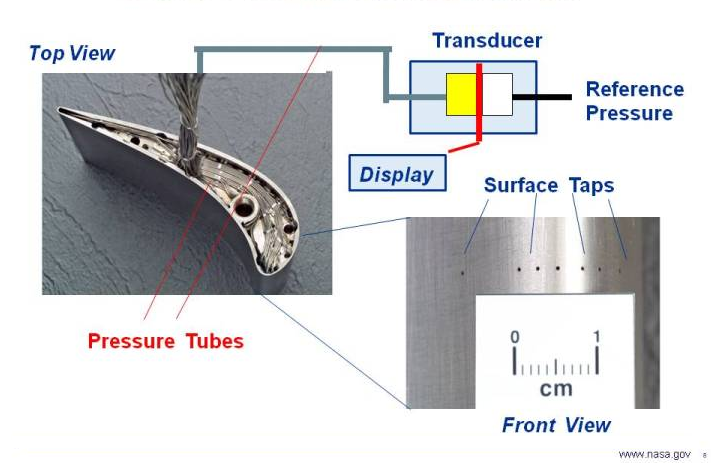
\includegraphics[width=0.5\textwidth]{figs/for_pres/taps.png} & 
            \centering
            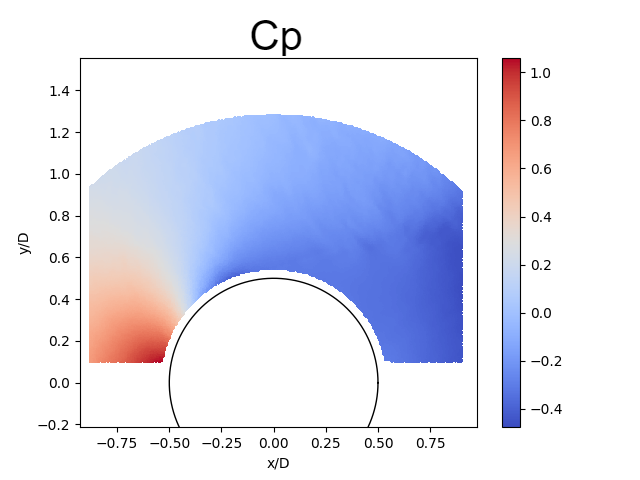
\includegraphics[width=0.5\textwidth]{figs/for_pres/cylinder_full.png}
        \end{tabular}
    \end{table}
\end{frame}

% Literature Review Slide
\section{Literature Review}
\begin{frame}{Motivation: Literature Review}
    \resizebox{\textwidth}{!}{
    \begin{tabular}{|c|c|c|c|}
        \hline
            Case         & Max Cp Error & Extrapolation Approach & Source                 \\
            \hline
            NACA 0012    & 0.5          & parabola fit           & Tagliabue et al., 2017 \\
            Sphere       & 0.15         & nearest neighbor       & Jux et al., 2020       \\
            Cyclist      & 0.2*         & nearest neighbor       & Jux et al., 2020       \\
            Bullet Step  & 0.02         & nearest neighbot       & Gent et al., 2018      \\
            NACA 0012    & 0.25         & line fit               & Ragni et al., 2009     \\
        \hline
    \end{tabular}
    }
    \footnotesize{*based on uncertainty analysis (no pressure tap reference)}
\end{frame}

% Issues Slide
\section{Issues with Extracting Surface Pressure}
\begin{frame}{Motivation: Issues with Extracting Surface Pressure}
    \begin{itemize}
        \item Reflections and low particle density
        \item Strong gradients due to curvature and boundary layer
    \end{itemize}
    \textbf{Goals:}
    \begin{itemize}
        \item Avoid extrapolation
        \item No numerical derivatives close to the wall
    \end{itemize}
\end{frame}

% Method Slide
\section{Method}
\begin{frame}{Method: Streamline Coordinates}
    \begin{center}
        \textbf{[Insert Streamline Diagram]}
    \end{center}
\end{frame}

\begin{frame}{Method: Summary}
    \begin{enumerate}
        \item Compute Streamlines
        \item Fit Circles
        \item Integration
        \item Differentiation
    \end{enumerate}
\end{frame}

% Results Slides
\section{Results}
\begin{frame}{Results: LES Airfoil}
    \begin{itemize}
        \item Data from Asada and Kawai, 2018
        \item Grid coarsened from LES
        \item Added 2\% random velocity error
    \end{itemize}
\end{frame}

\begin{frame}{Results: Rough Cylinder}
    \textbf{[Details and visualization]}
\end{frame}

\begin{frame}{Results: NACA 0018 (?)}
    \textbf{[Details and visualization]}
\end{frame}

% Conclusions Slide
\section{Conclusions and Next Steps}
\begin{frame}{Conclusions and Next Steps}
    \begin{itemize}
        \item Robust to noise
        \item Robust to distance from wall
        \item Similar or better results in regions with strong pressure gradient
    \end{itemize}
    \textbf{Next Steps:}
    \begin{itemize}
        \item Improve treatment of Reynolds stresses
        \item Improve treatment of critical points (separation, stagnation point)
        \item Generalization to 3D
    \end{itemize}
\end{frame}



\end{document}
